\subsection{Определение фокусных расстояний линз с помощью зрительной трубы}
\paragraph{Определение фокусного расстояния собирающих линз}


Настроим зрительную трубу на бесконечность
Поставим положительную линзу на расстоянии от предмета примерно равном фокусному. На небольшом расстоянии от линзы закрепим трубу, настроенную на бесконечность,
и отцентрируем её по высоте. Диафрагма диаметром $d = 1$ см, надетая на ближнюю к осветителю линзу, уменьшит сферические аберрации и повысит чёткость изображения.

Передвигая линзу вдоль скамьи, получим в окуляре зрительной трубы изображение предмета — миллиметровой сетки. При этом расстояние между предметом и серединой тонкой линзы (между проточками на оправах) равно фокусному.

    \begin{table}[h!]
      \caption{Результаты измерения фокусных расстояний линз}
        \centering
            \begin{tabular}{| c | c | c | c |}

                \hline
                    $n$ & $F_1, cm$ & $F_2, cm$ &  тип линзы\\
                \hline
                    1 & 8 & 8.2 & соб. \\
                \hline
                    2 & 10 & 10 & соб.\\
                \hline
                    3 & 18,8 & 19,3  & соб. \\
                \hline
                    4 & 32,5 & 32,5 & соб. \\
                \hline
                    5 & -9 & -9 &  рас.\\
                \hline
                \end{tabular}
        \label{nu1}
    \end{table}

\paragraph{Определение фокусного расстояния рассеивающей линзы}


Для определения фокусного расстояния тонкой отрицательной линзы сначала получим на экране увеличенное изображение сетки при помощи одной короткофокусной положительной линзы. Измерим расстояние между линзой и экраном $a_0 = 33.7$ см.
Разместим сразу за экраном трубу, настроенную на бесконечность, и закрпим её. Уберём экран и поставьте на его место исследуемую рассеивающую линзу (рис. 8). Перемещая рассеивающую линзу, найдите в окуляре зрительной трубы резкое изображение сетки. \par
Измерив расстояние между линзами $l = 24.7$ см, рассчитаем фокусное расстояние рассеивающей линзы $f = a_0 - l$.
Результаты измерения фокусного расстояния рассеивающих линз:

\begin{center}
    $f_{\text{рас}} = 33,7 - 24,7 \approx 9$ см
\end{center}


За погрешность измерений берем предел в 0.5 см, что логично из таблицы (1). Кроме того наложим ограничение в $0.05F$ для получения четкого изображения.

\begin{figure}[h!]
    \begin{center}
        \begin{minipage}[h!]{0.60\linewidth}
            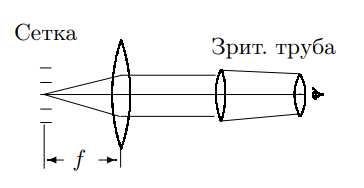
\includegraphics[width=1\linewidth]{plus_lens.png}
            \caption{Определение фокусного расстояния собирающей линзы}  подпись к рисунку
        \label{} 
        \end{minipage}

        \hfill 

        \begin{minipage}[h!]{0.60\linewidth}
            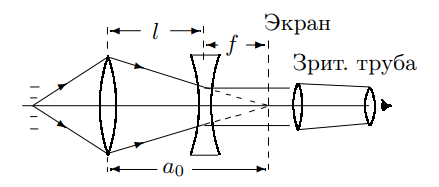
\includegraphics[width=1\linewidth]{minus_lens.png}
            \caption{Определение фокусного расстояния рассеивающей линзы}
        \label{}
    \end{minipage}
    \end{center}
\end{figure}
\newpage
\subsection{Моделирование трубы Кеплера}

Рассмотрим ход лучей в трубе Кеплера и найдём увеличение оптической схемы, изображеной 
на рисунке \ref{img::1}. Пусть пучок света, попадающий в объектив, составляет с оптической осью угол $\varphi_1$, а пучок, выходящий из окуляра, — угол $\varphi_2$. Увеличение $\gamma$ зрительной трубы по определению равно

\begin{equation}
    N = \frac{\tan \varphi_2}{\tan \varphi_1},
\end{equation}

но также из рис. \ref{img::3_3} следует, что :

\begin{equation}
    N_{\tau} = -\frac{f_1}{f_2} = -\frac{D_1}{D_2},
\end{equation}

где $D_1$ - ширина пучка, прошедшего через объектив, а $D_2$ - ширина пучка, вышедшего из окуляра

Построим оптическую систему из каллиматора и непосредственно трубы Кеплера. 

\begin{figure}[h!]
        \centering
            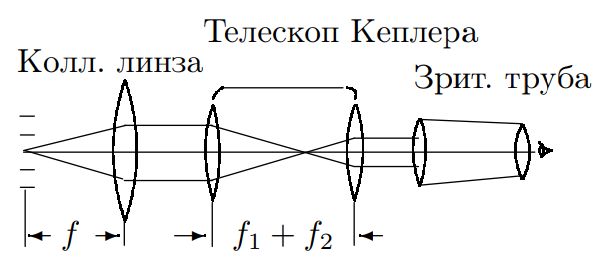
\includegraphics[width=10cm]{kepler_2.png}
            \caption{Схема трубы Кеплера}
        \label{img::3_3}
\end{figure}

Параметры действующих линз:

\begin{center}
    $f_{1} = 32.5$ см \hspace{1cm} $f_2 = 8$ см
\end{center}

Найдём увеличение трубы Кеплера непосредственно: пусть $h_1$ - размер ячейки миллиметровой сетки без телескопа, $h_2$ - с телескопом

\begin{center}
	$h_1 = 9$ мал. дел., \hspace{1cm} $h_2 = 34$ мал. дел. \par

	$N_{\tau} = -\frac{h_2}{h_1} \approx 3,7 \pm 0,53$
\end{center}

При этом по формуле (2) также

\begin{center}
    $N_{\tau} = -\frac{f_{1}}{f_2} \approx 4,06 \pm 0,51$
\end{center}

Кроме того существует еще один способ найти увеличение: частное $D_1 $ - диаметр объектива и $D_2$ - диаметр его изображения.

\begin{center}
	$N_{\tau} = -\frac{D_2}{D_1} = -\frac{3,4}{0,8} \approx -4,25 \pm 0,62$
\end{center}


\newpage
\subsection{Моделирование трубы Галилея}

Труба Галилея получается из трубы Кеплера заменой собирающей линзы окуляра рассеивающей. Формулы для увеличения, соответственно, остаются теми же:
\begin{equation}
    N_{\tau} = -\frac{f_1}{f_2} = -\frac{D_1}{D_2} =  -\frac{h_2}{h_1}
\end{equation}


Заменим собирающую линзу с фокусным расстоянием $f_2 = 8$ см рассеивающей с фокусным расстоянием $f_2 = 9$ см. Проведём те же операции, что и для трубы Кеплера:

\begin{center}
$h_1 = 9$ малых дел., \hspace{1cm} $h_2 = 30$ малых дел. \par
$N_{\tau} = -\frac{h_2}{h_1} \approx -3,33 \pm 0,46$
\end{center}

При этом выполняется так же:

\begin{center}
    $N_{\tau} = -\frac{f_1}{f_2} \approx -3,61 \pm 0,43$
\end{center}

Полученные значения хорошо совпадают.

\newpage
\subsection{Моделирование микроскопа}

Для создания модели микроскопа с увеличением $N_M = -5$ (минус, т.к. изображение перевернуто) отберём самые короткофокусные линзы из набора. 
Рассчитаем необходимый интервал $\Delta$ и длину тубуса  $l_12$ по формулам:

\[ N_m = -\frac{\Delta}{f_1} \cdot \frac{L}{f_2} \: \rightarrow \: \Delta = -\frac{N_m f_1 f_2}{L}  \]


Где $L = 25$ см - расстояние наилучшего зрения нормального. 


Получаем, что $\Delta = 16$ см. Затем $l_12 = \Delta + f_1 + f_2$ = 34 см.
Таким образом:

\[   N_m = -\frac{h_2 L}{h_1 f} = -\frac{31 \cdot 25}{9 \cdot 18,8} \approx -4,58  \pm 1,02  \]
